\documentclass[a4paper, 11pt, twoside]{article}
\usepackage{amssymb}
\usepackage{amsmath}
\usepackage{graphicx}
\begin{document}
\title{MATH6222 week 3 lecture 8}
\author{Rui Qiu}
\date{2017-03-09}

\maketitle

\paragraph{Problem:} L-tile, can a bunch of 3-unit area L-tiles admit a large L-shape with (100, 100, 50, 50, 50, 50)?\\

Bold conjecture: if the L-shape has an arrangement $L_n$ (edge length $2n$, removing the top right square part of length $n$). We could try to prove this by induction.\\

Let $P(n):= L_n$ admits an L-tiling.

But we cannot do $P(k-1)\implies P(k)$.

Suppose for a moment that $k$ is divisible by $3$. Then $2k$ is divisible by $3$. So $2k$ is not a multiple of $3$ so $2k-6$ is divisible by $3$.

.........\\

\textbf{check textbook page 61 and 62}.\\

The L-Tiling Problem. A child has a large number of L-shaped tiles as illustrated on the left below. Is it possible to form the large similar region on the right with non-overlapping copies of this tile?\\

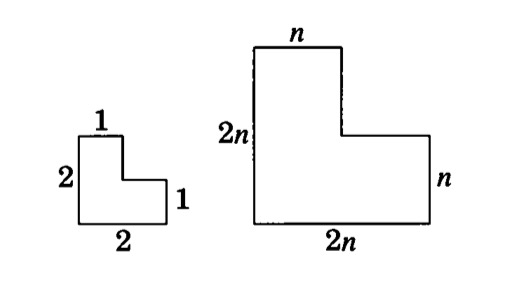
\includegraphics[width=\linewidth]{images/L1}

Let the large region be $R_n$ and the small region be $L$. A partition of a region into copies of $L$ is an \textbf{L-tiling}. We want to prove for $n\in\mathbb{N}$ that $R_n$ has an L-tiling. Since $R_1$ is a copy of $L$ itself, $R_1$ has an L-tiling.\\

In seeking a proof by induction, we can find a copy of $R_{n-1}$ inside $R_n$ by removing  a strip of unit width along the top, left, bottom, and right edges. This does not help. The induction hypothesis would tell us that  $R_{n-1}$ can be tiled, but when $n\geq 3$ we cannot extend this to a tiling of $R_n$ because the outer strip has no L-tiling.\\

To fix this flaw, we use an outer strip of width $2$ and obtain an L-tiling of $R_n$ from an L-tiling of $R_{n-2}$. Since $R_1$ has an L-tiling, this completes the proof for odd $n$, but to handle the even cases we also must treat $R_2$ in the basis. Below we explicitly tile $R_2$ and illustrate that every $2$ by $3k$ rectangle has an L-tiling. (The decomposition of $R_2$ suggests a simple inductive proof that $R_n$ has an L-tiling whenever $n$ is a power of $2$.)\\

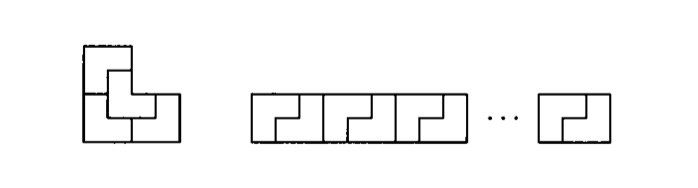
\includegraphics[width=\linewidth]{images/L2}

For the induction step, consider $R_n$, where $n\geq 3$. It suffices to cut $R_n$ into regions that we already know have L-tilings. The induction hypothesis provides an L-tiling of the inner region $R_{n-2}$. To complete the proof, it suffices to tile the outer strip. For this we use copies of $R_2$ and copies of $2$ by $3k$ rectangles, which we have already shown have L-tilings.\\

We tile the outer band in one of three ways, depending on whether $n, n-1,$ or $n-2$ is a multiple of $3$. To prove that the decomposition works in each case, we need only verify that the length of the long side of each rectangle used is a multiple of $3$. For clarity in the pictures, we list only these lengths; the short sides all equal 2. The three cases occur when $n\geq 3, n \geq 4$ and $n\geq 5$, respectively, so the lengths of the rectangles are nonnegative multiples of $3$. Verifying this completes the induction step.

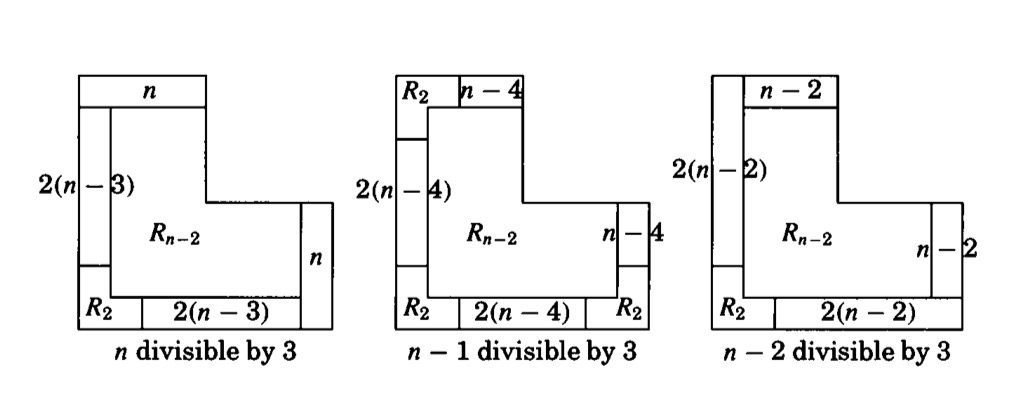
\includegraphics[width=\linewidth]{images/L3}

\paragraph{All horses are the same color (paradox)}

Base step: just one horse is trivial.\\

Inductive step: Assume that $n$ horses always are the same color. Let us consider a group consisting $n+1$ horses.\\

First, exclude the last horse and look only at the first $n$ horses; all these are the same color since $n$ horses always are the same color. Likewise, exclude the first horse and look at the last $n$ horses. These too, must also be of same color. Therefore, the first horse in the group is of the same color as the color as the horses in the middle, who in turn are of the same color as the last color. Hence the first horse, middle horse, and last horse are all of the same color, and we have proven that:

\[\text{If } n \text{ horses have the same color, then } n+1 \text{ horses will also have the same color.}\]

We already saw in the base case that the rule ("all horses have the same color") was valid for $n=1$. The inductive step showed that since the rule is valid for $n=1$, it must also be valid for $n=2$, which in turn implies that the rule is valid for $n=3$ and so on.\\

Thus in any group of horses, all horses must be the same color.\\

Explanation: The argument above makes the implicit assumption that the two subsets of horses to which the induction assumption is applied have a common element. This is not true when the original set (prior to either removal) only contains two horses.\\

Let the two horses be horse A and horse B. When horse A  is removed, it is true that the remaining horses in  the set  are the same color (only horse B remains). The same is true when horse B is removed. However the statement "the first horse in the group is of the same color as the horses in the middle" is meaningless, because there are no "horses in the middle" (common elements (horses) in the two sets). Therefore the above proof has a logical link broken. The proof forms a falsidical paradox; it seems to show by valid reasoning something that is manifestly false, but in fact the reasoning is flawed.\\

\end{document}